\begin{center}
  \Large
  \textbf{BIOGRAFI PENULIS}
\end{center}

\addcontentsline{toc}{chapter}{BIOGRAFI PENULIS}

\vspace{2ex}

\begin{wrapfigure}{L}{0.3\textwidth}
  \centering
  \vspace{-3ex}
  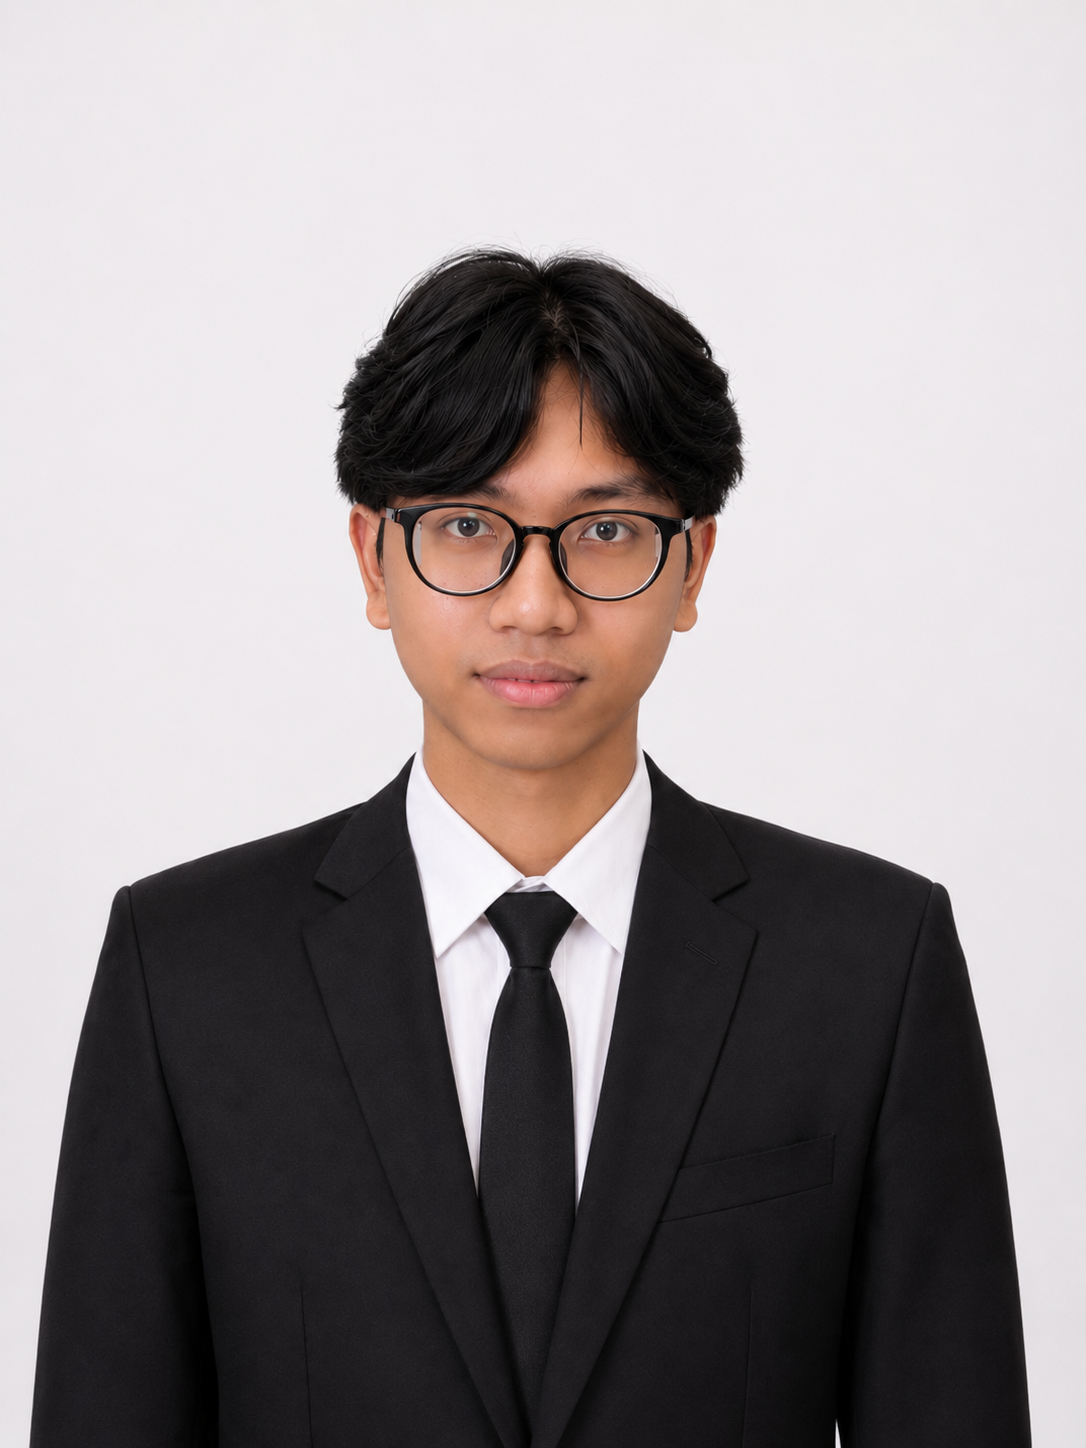
\includegraphics[width=0.3\textwidth]{gambar/foto.png}
  \vspace{-4ex}
\end{wrapfigure}

Penulis bernama Priagung Ramadhan Alfalakhi, lahir di Jombang pada tanggal 02 November 2003. Penulis merupakan mahasiswa Program Studi Sarjana Teknik Elektro, Departemen Teknik Elektro, Institut Teknologi Sepuluh Nopember (ITS), Surabaya. Selama menempuh pendidikan di ITS, penulis aktif mengikuti berbagai kegiatan akademik maupun non-akademik sebagai sarana pengembangan kompetensi, kepemimpinan, serta kemampuan bekerja sama dalam tim.

Dalam bidang akademik, penulis terlibat dalam berbagai proyek penelitian dan pengembangan yang mencakup sistem robotika, sistem monitoring, computer vision, machine learning, serta berbagai proyek berbasis perangkat keras dan perangkat lunak lainnya. Selain melalui kegiatan penelitian, penulis juga memperoleh pengalaman melalui berbagai proyek perkuliahan serta pengembangan robot untuk kebutuhan kompetisi. Pengalaman tersebut memberikan pemahaman yang lebih luas mengenai penerapan teknologi dalam menyelesaikan permasalahan nyata.

Pada bidang organisasi dan pengembangan diri, penulis aktif berpartisipasi dalam berbagai kegiatan kepanitiaan, khususnya pada divisi administrasi dan perlengkapan. Penulis juga aktif dalam kegiatan Himpunan Mahasiswa Teknik Elektro ITS, mulai dari posisi staf hingga dipercaya mengemban amanah sebagai Kepala Departemen Lingkungan dan Pengabdian Masyara\-kat. Selain itu, penulis turut berkontribusi sebagai asisten laboratorium, dimulai sebagai staf asisten hingga menjabat sebagai Asisten Koordinator.

Penulis juga memperoleh pengalaman profesional melalui program magang di Badan Riset dan Inovasi Nasional (BRIN). Pada kegiatan tersebut, penulis terlibat dalam pengembangan sistem yang berkaitan dengan teknologi kendaraan otonom, sejalan dengan bidang penelitian yang diangkat dalam tugas akhir ini.

Bidang yang paling diminati oleh penulis adalah \textit{computer vision}, khususnya pada penerapan metode deteksi dan segmentasi untuk robot maupun kendaraan otonom. Penulis meyakini bahwa teknologi kecerdasan buatan dan sistem persepsi cerdas akan memiliki peran penting dalam perkembangan robotika dan transportasi masa depan. Oleh karena itu, penulis berharap dapat terus berkontribusi dalam pengembangan teknologi yang bermanfaat bagi masyarakat. Melalui penelitian tugas akhir mengenai navigasi robot beroda otonom berbasis logika fuzzy menggunakan LiDAR dan kamera termal, penulis berharap hasil yang diperoleh dapat memberikan kontribusi positif bagi pengembangan teknologi navigasi otonom dan menjadi referensi bagi penelitian selanjutnya.